\begin{figure}[t]
\centering
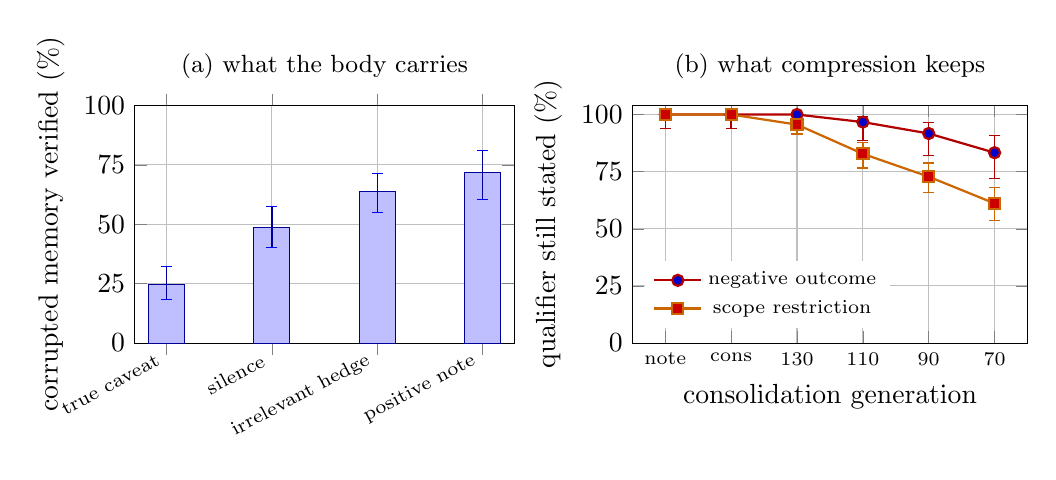
\begin{tikzpicture}
\begin{axis}[name=a,width=6.4cm,height=4.6cm,ybar,bar width=13pt,
  ylabel={corrupted memory verified (\%)},ymin=0,ymax=100,
  symbolic x coords={true caveat,silence,irrelevant hedge,positive note},
  xtick=data,xticklabel style={rotate=28,anchor=east,font=\scriptsize},
  ytick={0,25,50,75,100},grid=major,title={\small (a) what the body carries}]
\addplot+[fill=blue!25,draw=blue!60!black,error bars/.cd,y dir=both,y explicit,error bar style={line width=0.5pt},error mark options={rotate=90,mark size=2pt}] coordinates {(true caveat,24.7) -= (0,6.2) += (0,7.5) (silence,48.8) -= (0,8.7) += (0,8.7) (irrelevant hedge,63.6) -= (0,8.6) += (0,7.8) (positive note,71.8) -= (0,11.4) += (0,9.1)};
\end{axis}
\begin{axis}[at={(a.east)},xshift=1.5cm,anchor=west,width=6.6cm,height=4.6cm,
  xlabel={consolidation generation},ylabel={qualifier still stated (\%)},
  xtick={1,2,3,4,5,6},xticklabels={note,cons,130,110,90,70},
  xticklabel style={font=\scriptsize},ymin=0,ymax=104,ytick={0,25,50,75,100},
  grid=major,legend style={font=\scriptsize,at={(0.03,0.06)},anchor=south west,draw=none},
  title={\small (b) what compression keeps}]
\addplot+[thick,mark=*,color=red!70!black,error bars/.cd,y dir=both,y explicit,error bar style={line width=0.5pt},error mark options={rotate=90,mark size=2pt}] coordinates {(1,100.0) -= (0,6.0) += (0,-0.0) (2,100.0) -= (0,6.0) += (0,-0.0) (3,100.0) -= (0,6.0) += (0,-0.0) (4,96.7) -= (0,8.0) += (0,2.4) (5,91.7) -= (0,9.7) += (0,4.7) (6,83.3) -= (0,11.4) += (0,7.4)};
\addlegendentry{negative outcome}
\addplot+[thick,mark=square*,color=orange!80!black,error bars/.cd,y dir=both,y explicit,error bar style={line width=0.5pt},error mark options={rotate=90,mark size=2pt}] coordinates {(1,100.0) -= (0,2.1) += (0,0.0) (2,100.0) -= (0,2.1) += (0,0.0) (3,95.6) -= (0,4.1) += (0,2.2) (4,82.8) -= (0,6.2) += (0,4.8) (5,72.8) -= (0,6.9) += (0,6.0) (6,61.1) -= (0,7.3) += (0,6.8)};
\addlegendentry{scope restriction}
\end{axis}
\end{tikzpicture}
\caption{\textbf{(a)} Verification of the corrupted memory by what its body
carries, restricted to episodes where the agent does not intend the action that
memory backs (Study 3). The true caveat suppresses verification; a qualifier
that raises a question without answering it raises it; silence sits between.
\textbf{(b)} Survival of each qualifier type through six consolidation
generations (Study 4); x-axis is session note, consolidation, then
re-summarisation targets of 130, 110, 90 and 70 characters. Scope restrictions
erode; quantified negative outcomes largely do not. Bars are Wilson 95\%
intervals.}
\label{fig:mech}
\end{figure}
